\documentclass[final,t]{beamer}
\mode<presentation>{
  \usetheme{CPTposter}
}
\usepackage{ragged2e}

% additional packages
\usepackage{listings}
\usepackage{amsmath,amsthm, amssymb, latexsym}
\usepackage{exscale}
\usepackage[orientation=portrait,size=a0,scale=0.8]{beamerposter}
\usepackage{tikz}
\usetikzlibrary{shapes,arrows}
\usepackage{multirow}



\title{Enhancing Student Engagement with Online Annotation of Bacteriophage Genomes}
\author{\huge Eric Rasche$^{\text{1}}$, Jason Gill$^{\text{2}}$, Ryland Young$^{\text{1, 3}}$}
\institute{\Large %
1. Center for Phage Technology, Texas A\&M University, College Station, United States\\%
2. Department of Animal Science, Texas A\&M University, College Station, United States\\%
3. Department of Biochemistry and Biophysics, Texas A\&M University, College Station, United States}

% abbreviations
\setlength\parindent{1cm}

\begin{document}
\begin{frame}[fragile]
    \vspace{-.8cm}
    \begin{columns}[t]
        \columnPadding{0.00}
        \begin{column}{.36\linewidth}

            \begin{block}{BICH464: Phage Genomics for undergraduates}
                1 semester, 3 credit course taught for 12 years (pre-dates HHMI Phage Hunters). Each student:
                \begin{itemize}
                    \item Annotates a complete, novel phage genome in 1 semester
                    \item Prepares and polishes a Genbank file for submission
                    \item Writes a 500 word submission for ASM Genome Announcements
                \end{itemize}
                The students additionally isolate novel phages from the environment for future years.

                The ultimate goal of the course is student exposure to real research,
                including the time demands, requirement for initiative,
                intense phage biology, and fundamental genomics required.
            \end{block}



            \begin{block}{Why Undergraduate Phage Genomics?}
                \begin{itemize}
                    \item Phages are ideal--small size, high coding
                        density
                    \item Can be annotated within a single semester, by a
                        single undergraduate
                    \item Sequencing and assembly are no longer the
                        throughput-limiting step.
                \end{itemize}
            \end{block}

            \begin{block}{Previous Course Iterations}
                \justifying
                Students
                \begin{itemize}
                    \item Students hated the command line!
                    \item Struggled to copy command line statements and failed
                        to understand the relationship between their printed
                        protocols and their screen.
                \end{itemize}
                Staff
                \begin{itemize}
                    \item Documenting parameters students used in
                        software was impossible (typos, closed-source websites).
                    \item Dependence on mutable third party services was
                        quite problematic for reproducibility.
                \end{itemize}

                These issues resulted in sub-optimal experience for everyone
                involved, and some steps were not strictly reproducible.
            \end{block}

            \begin{block}{CPT Viral Annotation Innovations}
                Use Galaxy
                \begin{itemize}
                    \item Galaxy provides a single interface to all software,
                        from BLAST to InterProScan to TMHMM.
                    \item Galaxy is a robust system with extremely large community
                        supporting development and features. Not just for eukaryotic genomics!
                    \item \emph{100\% reproducible science.}
                    \item Automatic tracking of user's files and tool run history.
                    \item Perfect documentation of commands run and parameters used.
                \end{itemize}
                Workflows!
                \begin{itemize}
                    \item Students run complete, automated workflows instead of
                        running individual tools, or typing in complex command
                        line statements.
                    \item Everyone runs identical workflows, and admins can
                        pre-configure steps, eliminating user error rate.
                    \item More time for teaching and bioinformatics.
                \end{itemize}
                Apollo is the Future
                \begin{itemize}
                    \item Leverages a widely used system with large community
                        for annotation of viral organisms.
                    \item Students only see the most up-to-date copy, which we
                        transparently and automatically back up.
                    \item Students cannot lose files or progress. They cannot
                        accidentally switch to an old version.
                    \item Unified display of outputs of very different tools.
                \end{itemize}
            \end{block}

            \begin{block}{Current Status \& Future Plans}
                Try it Today! \url{https://cpt.tamu.edu/beta}
                \begin{itemize}
                    \item Open Beta for Galaxy \& Apollo annotation workflow.
                    \item All work is open source, and community-focused.
                    \item NSF funding for further development of community
                        viral annotation (\emph{de novo} and re-annotation) efforts.
                \end{itemize}
                Future
                \begin{itemize}
                    \item Easily clone our infrastructure, and deploy your own
                        annotation community!
                \end{itemize}
            \end{block}

        \end{column}
        \columnPadding{0.00}
        \begin{column}{.60\linewidth}
            \begin{block}{Galaxy \& Apollo: Automation \& Unified Results Display }
                \begin{figure}
                    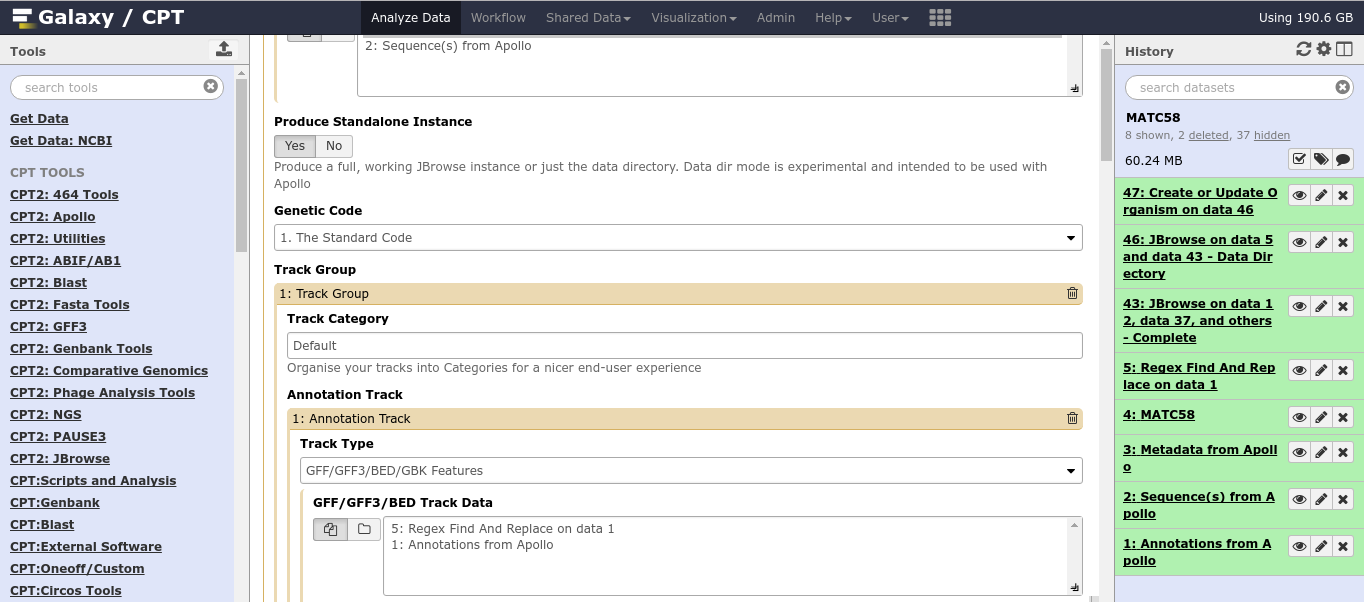
\includegraphics[width=0.98\textwidth]{./media/galaxy.png}
                    \caption{In \textbf{Galaxy}, every tool has a standardized
                        interface. Once students learn the interface, they can
                        use any of the $\approx$600 tools available in the
                        CPT's Galaxy, just by understanding the tool's use
                        case. Tool runs are automatically recorded in their
                        \emph{history}, like an automated lab notebook.}
                \end{figure}
                \begin{figure}
                    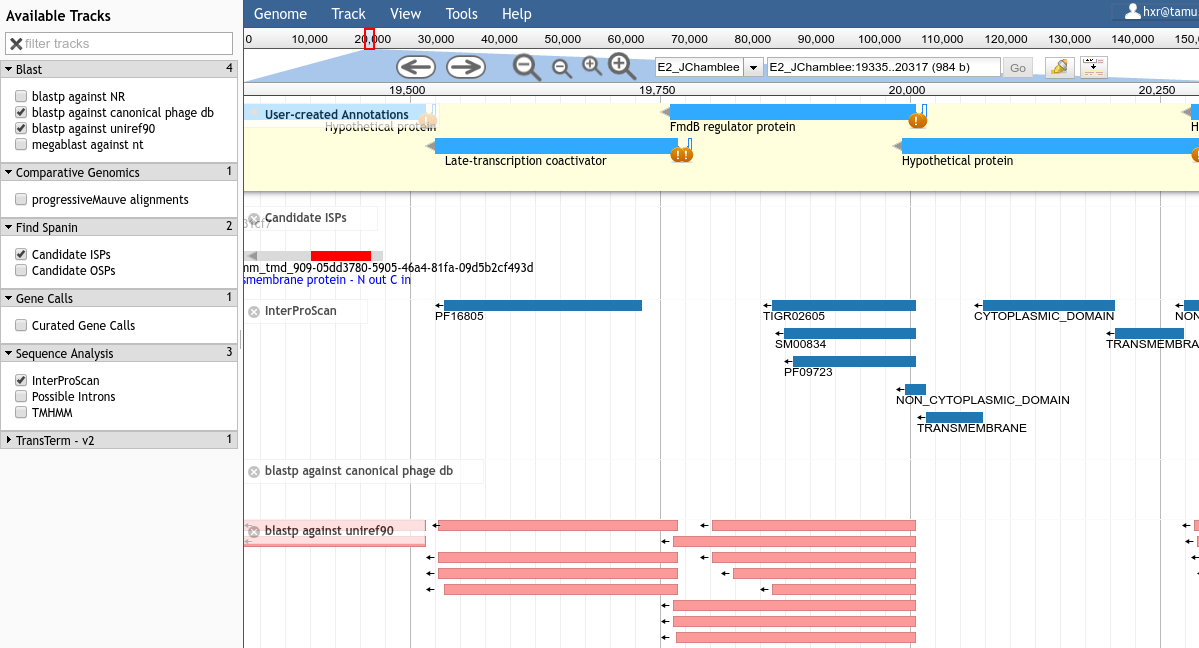
\includegraphics[width=0.98\textwidth]{./media/apollo.png}
                    \caption{\textbf{Apollo}, the online, real-time,
                    collaborative genome annotation suite, has significantly
                    increased student/staff productivity and
                    decreased IT burden. Results from highly disparate HTML
                    pages, text files, blast reports, etc. are visually
                    unified, allowing researchers to focus on biology rather
                    than on interpreting reports.}
                \end{figure}

                \begin{figure}
                    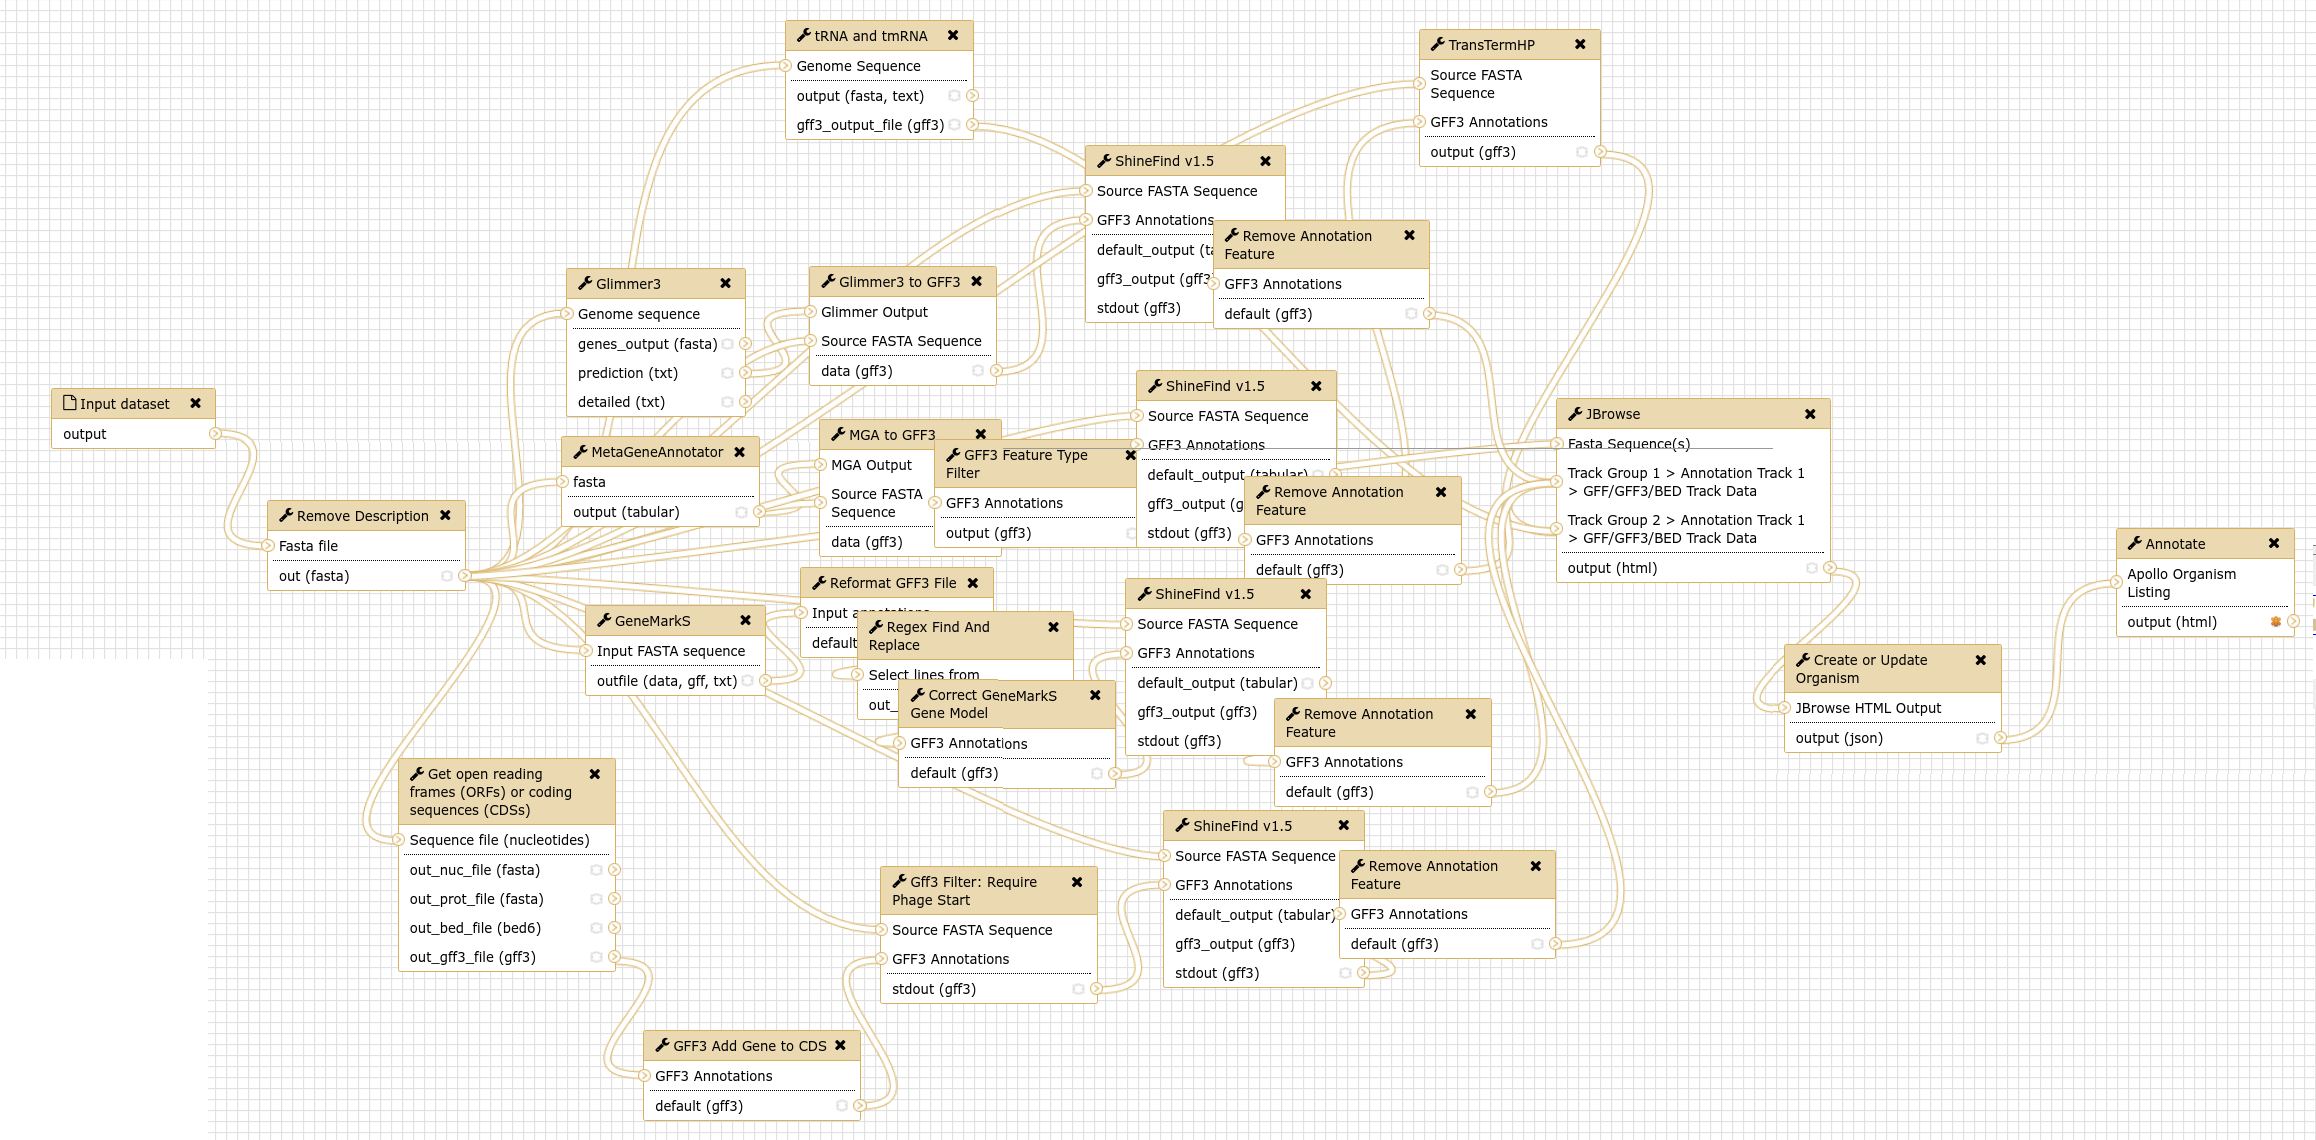
\includegraphics[width=\textwidth]{./media/workflow.png}
                    \caption{Galaxy Workflows enable researchers to develop
                    common analysis units such as ``Gene Calling'', and to
                    adjust these workflows whenever new and improved methods
                    become available. We recently added MetaGeneAnnotator to our
                    gene callers. Students and researchers could then
                    compare identically-styled GeneMarkS, Glimmer3, and MGA
                    outputs in Apollo. They could bypass the opaqueness of
                    large text reports, and cut right to the biology.}
                    \vspace{-0.3cm}
                \end{figure}
            \end{block}
        \end{column}
  \end{columns}
\end{frame}
\end{document}
